\section{Architectural Design}
\subsection{Overview}
We chose the three tier architecture for S\&C. We believe that it is a solid choice aligned with our goals and requirements. \\
The architecture is divided in three:
\begin{enumerate}
    \item\textbf{Presentation Tier} \\
    This is essentially the user interface
    \item\textbf{ Application Tier} \\
    This layer is where the data are transformed and undergo a set of processes to make them available to the user interface
    \item\textbf{Data Tier} \\
    This layer is where the data are stored and managed remotely.
\end{enumerate}
\begin{figure}[h!]
        \centering  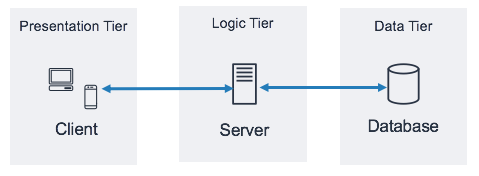
\includegraphics[width=1\textwidth]{DD/Images/aws.png}
        \label{fig:CompleteStudentProfile}
\end{figure}
The choice of implementing a three-tier architecture has several advantages.
\begin{itemize}
    \item The various tiers can be developed simultaneously and independently by different people or teams of people making the development phase faster
    \item The division in three tiers makes the separation of different functions more clear and makes the code easier to be understood and maintained
    \item The separation in three allows each layer to be scaled independently from the others, thus enhancing the overall scalability of the web application
\end{itemize}
\subsection{Component View}
The main components of the back-end are:
\begin{itemize}
    \item \textbf{SearchManager}: it is the component in charge of receiving and handling the search requests about the internship positions issued by the students 
    \item \textbf{RegistrationManager}: it is the component in charge of managing the registration of the users.
    \item \textbf{LoginManager}: it is the component in charge of the login of the users
    \item \textbf{NotificationManager}: it is the component in charge of sending the notifications to users, including push notifications and confirmation emails used to validate email accounts in the registration process
    \item \textbf{ProfileManager}: it is the component in charge of handling user profile information. It is supposed dot interact with all the other components in order to keep the profile of the user up to date.
    \item \textbf{InternshipManager}: it is the component in charge of managing the internships. It manages the internship status, the communication, the assessment process (if needed), publishing of news related to the internships.
    \item \textbf{ApplicationManager}: it is the component in charge of keeping track of the status application and its details.
    \item \textbf{API}: it is the component that allows the back-end to interact with the requests from the front-end.
    \item \textbf{WebApp}: it is the component in charge of providing the user interface for interacting with the system. It relies on the API to fetch and send data for various operations.
    \item \textbf{Database}: it is the component in charge of storing all the information relevant to the platform.
\end{itemize}
\begin{figure}[h!]
        \centering  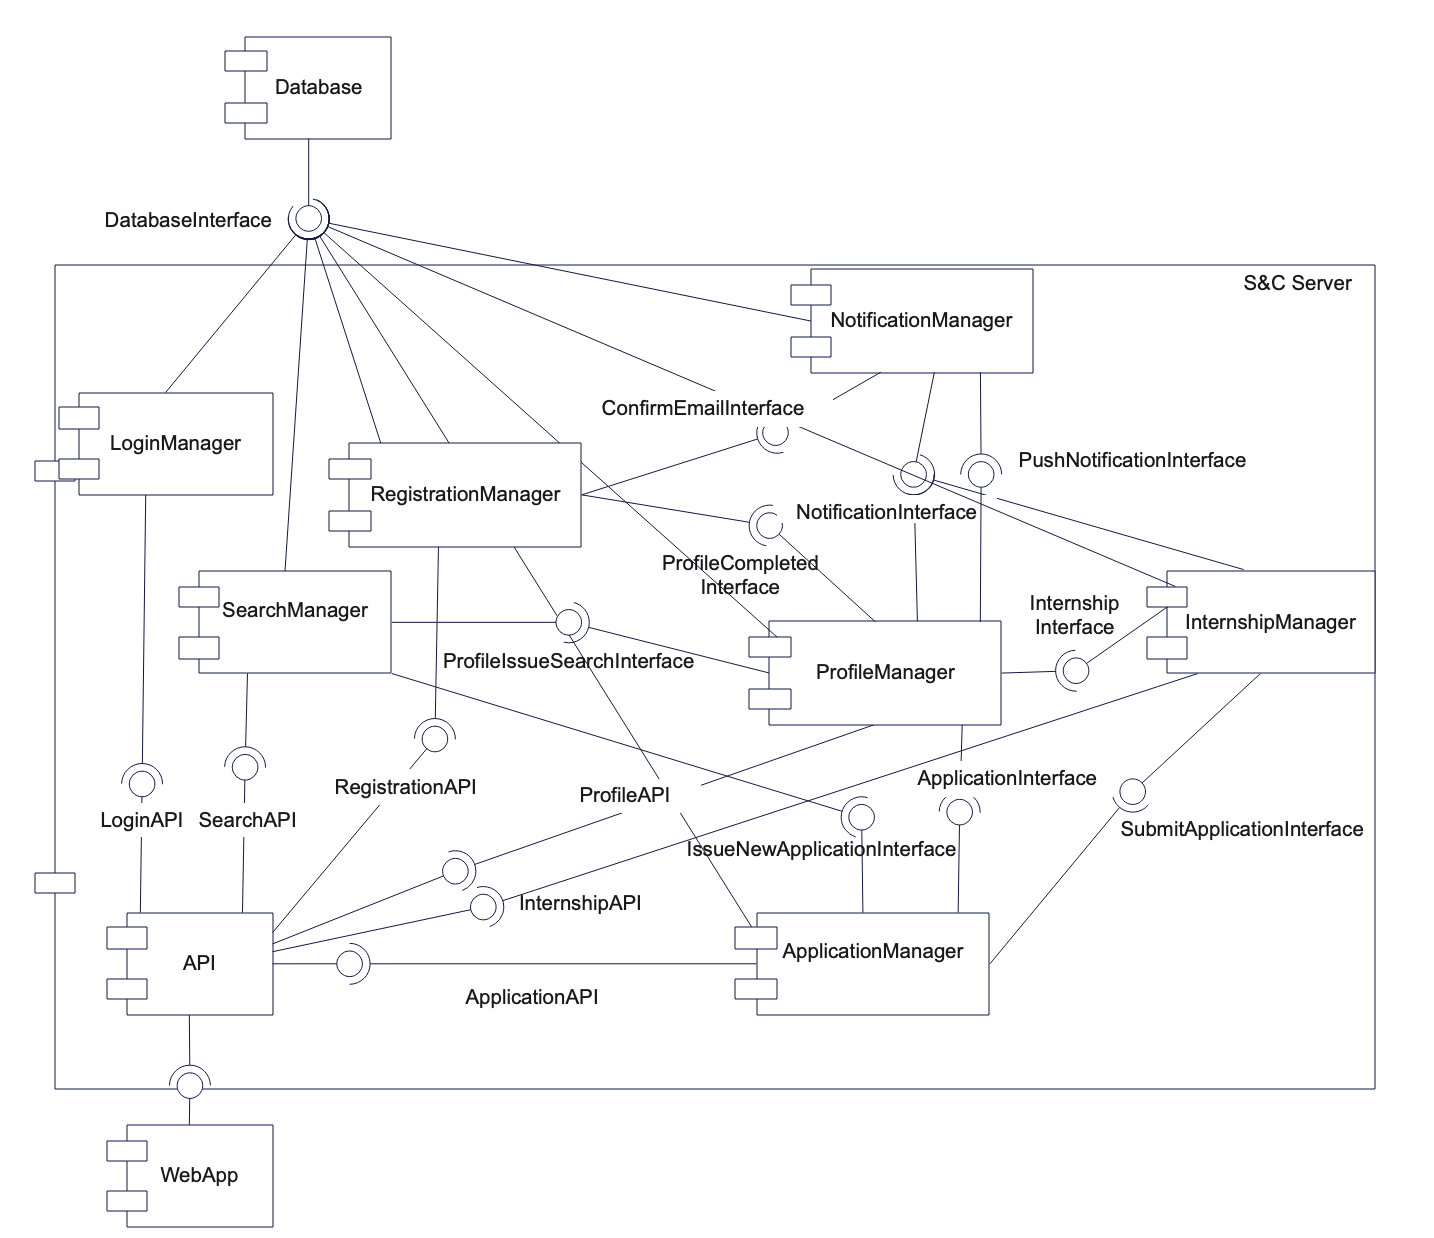
\includegraphics[width=1\textwidth]{DD/Images/ComponentViewDiagram.png}
        \label{fig:ComponentViewDiagram}
\end{figure}

